\chapter{Toolchain Usage}
The twill toolchain is made up of complex pieces of software, each communicating with the others. As such the workflow involved in getting through the tool chain is not negligable just yet.

\section{LLVM Compilation}
The compiler portion of Twill is mostly all automated by a python script, that takes in only a few options. 

\subsection{Running the Python Script}
Figure [[TODO: INSERT FIGURE SHOWING EXAMPLE OF PYTHON EXECUTION]] shows an example invocation of the script. The second argument is the target C file that you want to run through the toolchain. This file should contain the ``main'' function for the program in order for the toolchain to compile correctly. The first argument to the script is the number of partitions you want created. Currently, using 1 for this parameter will not generate any hardware, while using 2 will generate the hardware partition. In theory higher numbers will still function, generating more hardware partitions, though this functionality has not been tested, and may require additinonal changes elsewhere.

The python script takes the input file, and then runs it through the compilation path that is described in the original Twill paper [TODO: INSERT TWILL REFERENCE HERE]. After running through all the LLVM passes, the python script will copy the generated software and hardware files into the appropriate location of a Xilinx project. 

\section{Xilinx}
After running the python script runs, the rest of the tool chain lies within Xilinx ISE, which is responsible for synthesizing the hardware, and uploading and running the code on the actual hardware.

\subsection{Xilinx ISE}
After running the python script, Xilinx ISE can be opened up to the ``uHTheadsCustom'' project. This project contains a pre-generated MicroBlaze processor, the hardware software interface HDL, and should already include the generated hw file. The next step in the process is to synthesize the top level module, the uHThreads object. This will synthesize the generated hardware, the processor, and the glue logic between the two generating a bitstream. After synthesis is complete, the hardware design should be exported to Xilinx SDK with the bitstream.

\subsection{Xilinx SDK}
Exporting the bitstream will open up the Xilinx SDK, which is based on Eclipse. There should be 2 projects open here, one that contains the BSP for the target FPGA device, and the uHThreadsCode project, which is where the software portion from the python script was copied earlier. In main.c, the main function initializes the Twill runtime, starts up the hardware threads, and then executes the program. After execution the number of cycles taken to execute the program and the return value from the ``main'' function in the original program will print over a Serial connection.

To actually program the FPGA, ensure that the hardware is connected to the host, typically through a JTAG connection. Click the ``Program FPGA'' which will display the dialog shown in Figure \ref{fig:fpga_diag_box}.

\begin{figure}
	\centering
		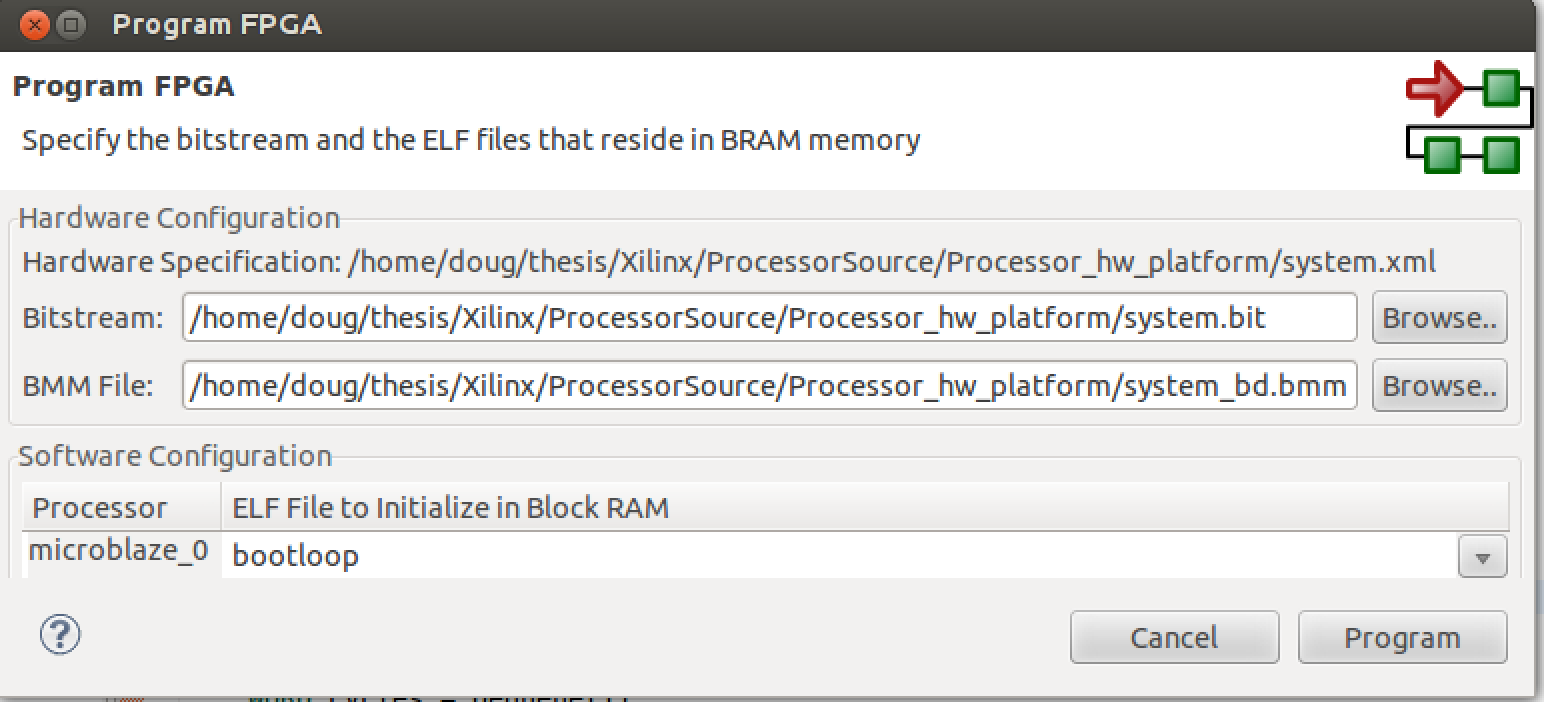
\includegraphics[width=\textwidth]{figures/fpga_diag_box}
	\caption{Program FPGA Dialog Box\label{fig:fpga_diag_box}}
\end{figure}

Ensure that the ``.bit'' file and ``.bmm'' file correspond to the correct files in the board support project, and then click program to upload the program to the FPGA. After the program is finished uploading, you should be able to click the debug button which will launch the debug view and allow you to debug, or run through the program as necessary. 